
%mainfile: Multimodal_learning.tex

\title{Multimodal Learning: Examples in Gesture and Audio-Visual
Speech Recognition\vspace{-0.5em}}
\author{Hsieh Yu-Guan}
\date{\today}
\maketitle

\section*{Abstract}

\section{Introduction}

\section{Related Work}

\section{Presentation of Basic Network Architectures}

\subsection{Conolutional Neural Networks}

Convolutional Neural Networks (CNNs) are an early family of deep learning
architectures inspired from the human vision system \cite{Y. LeCun 1998}.
Generally we have convolutional layers alternating with pooling
(subsamping) layers, but fully connected layers can also be introduced.
CNNs have been shown to achieve state-of-the-art performance in
image processing tasks such as image classification
\cite{A. Krizhevsky 2012} and object detection \cite{Y. LeCun 2010}.
However they can be equally applied in other fields like speech recogntion
\cite{L. Deng 2013}.

\subsection{Auto-encoder}

Auto-encoders are networks that are trained to minimize the reconstruction
error by back-propagating it from the output layer to hidden layers.
In the simplest model with one hidden layer, an auto-encoder takes an
input $\mathbf{x} \in \mathbb{R}^d$ and maps it to the latent
representation $\mathbf{h} \in \mathbb{R}^{d'}$ given by
$\mathbf{h} = \sigma(W\mathbf{x}+\mathbf{b})$ where $W$
is a weight matrix, $\mathbf{b}$ is a bias vector and $\sigma$ is an
activation function. Then the network tries to reconstruct the input
by a reverse mapping $\mathbf{x'} = \sigma(W'\mathbf{h}+\mathbf{b'})$.

To prevent the auto-encoder from learning the identity function as
a trivial solution, several regularization techniques have been proposed.
The bottleneck approach forces dimensionality reduction by having
fewer neurons in hidden layers than in the input layer. For example,
in the above case, we must have $d'<d$. Sparse auto-encoders impose sparsity
on hidden units \cite{A. Makhzani 2014}.
Denoising auto-encoders, which play an important role in my internship,
try to recontruct the clean input from its corrupted version
\cite{P. Vincent 2008, Y. Bengio 2012}. Binomial noise
(switching pixels on or off) adding
to input or hidden layers are used in my case.

Intuitively, auto-encoders are useful for data reconstruction.
Nevertheless, the true interest lies in fact in its capcity to learn
a representation (encoding) for a set of data in a purely unsupervised
fashion \cite{P. Vincent 2010}. Recently, auto-encoders are also
more and more often used as a generative model \cite{Y. Bengio 2013}.

\section{Datasets and Preprocessing}

Many datasets were explored during my internship. The three main datasets
being used are given in details  below. Two of them are for gesture
recognition:
Creative Senz3D \cite{A. Memo 2015, A. Memo 2017} and ASL Finger Spelling
\cite{N. Pugeault 2011}, and one is for AVSR: AVLetters
\cite{I. Matthews 2002}.

\subsection{Creative Senz3D}

The dataset contains gestures perfomed by 4 different people, each
performing 11 different static gestures repeated 30 times each,
for a total of 1320 samples.
For each sample, color, depth and confidence frames are available.
I only used the color and depth frames of this dataset. The original
size of each image is $480 \times 640$ and they're resized to
$299 \times 299$ pixels before being fed to the network. No other
preprocessing are done. For both color and depth images I use the three
color channels (even though a priori only one channel is needed for
depth maps).

\begin{figure}[H]
  \centering
  \hfill
  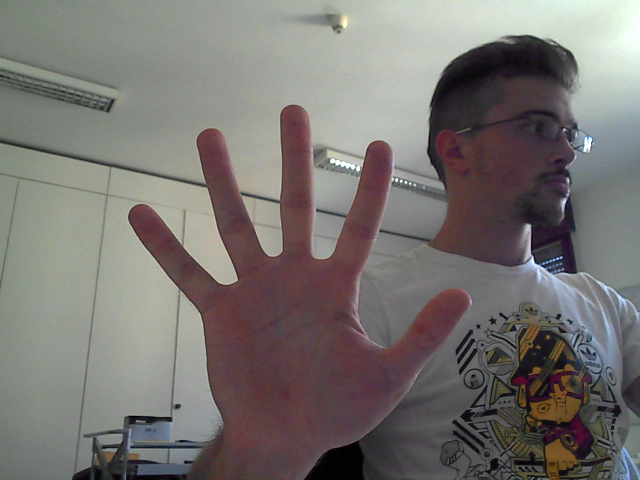
\includegraphics[width=0.23\linewidth]{dataset/senz3d/examples/1-color}
  \hfill
  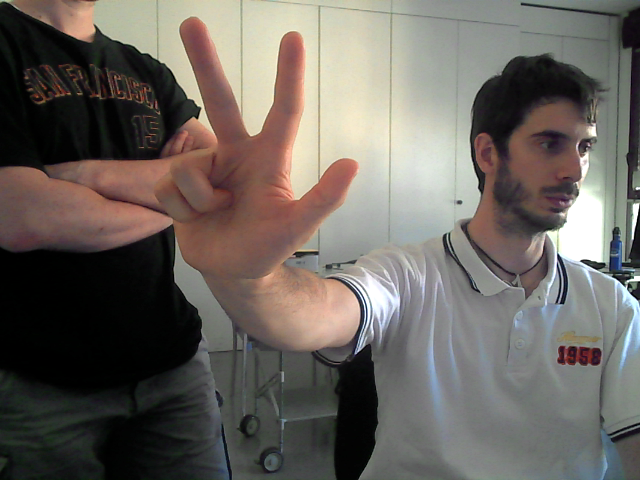
\includegraphics[width=0.23\linewidth]{dataset/senz3d/examples/12-color}
  \hfill
  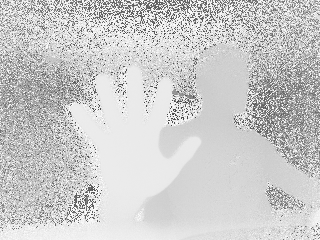
\includegraphics[width=0.23\linewidth]{dataset/senz3d/examples/1-depth}
  \hfill
  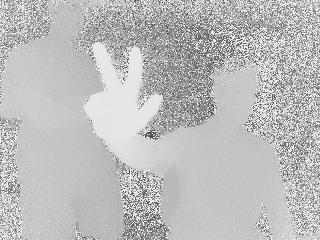
\includegraphics[width=0.23\linewidth]{dataset/senz3d/examples/12-depth}
  \caption{%
    \textbf{Example images in the Creative Senz3D dataset.}\\[0.1em]
    Left Two) Color images.\\[0.1em]
    Right Two) Corresponding depth images.\\[0.1em]
    All of the images are of size $480 \times 640$ and contain the
      the entire upper body of the subject.}
  \label{fig:senz3d_exs}
\end{figure}

\subsection{ASL Finger Spelling}

The dataset is composed of more than 60000 images in each modality
(RGB and depth images are provided).
Five subjects are asked to perform the 24 static signs in
the American Sign Language (ASL) alphabet (excluding j and z which involve
motion) a certain number of times, captured with similar lighting
and background.

Images of this dataset are of variable sizes. The data preprocessing
includes resizing each image to $83 \times 83$ pixels,
converting to grayscale and adjusting
contrast of depth maps. Only very late in my internship I added the
Z-normalization (normalize to zero mean and unit of variance)
as a preprocessing step and the only result that was largely changed
is presented in \ref{subsection:CAE}.

\begin{figure}[H]
  \centering
  \hfill
  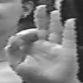
\includegraphics[width=0.15\linewidth]{%
    dataset/fingerspelling5/exs/or/g1}
  \hfill
  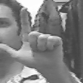
\includegraphics[width=0.15\linewidth]{%
    dataset/fingerspelling5/exs/or/g2}
  \hfill
  
\includegraphics[width=0.15\linewidth]{%
    dataset/fingerspelling5/exs/or/d3}
  \hfill
  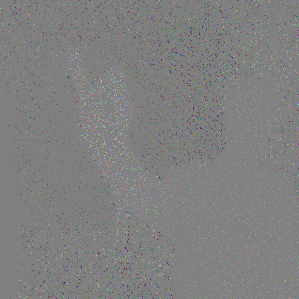
\includegraphics[width=0.15\linewidth]{%
    dataset/fingerspelling5/exs/or/d4}
  \hfill
  
\includegraphics[width=0.15\linewidth]{%
    dataset/fingerspelling5/exs/st/d1}
  \hfill
  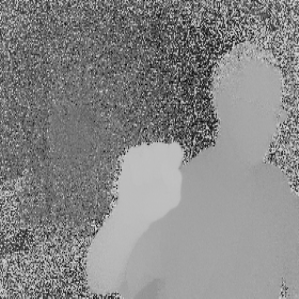
\includegraphics[width=0.15\linewidth]{%
    dataset/fingerspelling5/exs/st/d2}
  \caption{%
    \textbf{Example images in the ASL Finger Spelling dataset
      (after preprocessing).}\\[0.1em]
    Left Two) Grayscale intensity images.\\[0.1em]
    Middle Two) Depth maps after adjusting contrast.\\[0.1em]
    Right Two) Depth maps after Z-normalization.\\[0.1em]
    Images of this dataset have variable sizes, and they're all resized to
      $83 \times 83$ before being fed to the network. Generally only the
      hand region is contained in image.}
  \label{fig:fingerspelling_exs}
\end{figure}

\subsection{AVLetters}

The dataset comprises video and audio recordings of 10 speakers
uttering the letters A to Z, three times each.
We count therefore 780 samples in total. For video data, image sequences
of pre-extracted lip regions are provided.
Each single image if of size $60 \times 80$.
For audio data, only the mel-frequency cepstrum coefficients (MFCCs)
are given, and each audio frame is represented by 26 mfccs.
The lack of raw audio data is a strong constraint on what we're able to do
on this dataset.

Since all utterances don't have the same time duration, I used
fourier resamping to force every video input to be of length 12 and
every audio input to be of length 24. Video frames are Z-normalized.
Several data augmentation techniques
are also considered, including random brightness adjusting, random contrast
adjusting and random cropping (but at least 80\% of the original image
is kept).

\begin{figure}[H]
  \centering
  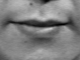
\includegraphics[width=0.15\linewidth]{%
    dataset/avletters/lips_no_data_aug/1}
  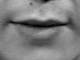
\includegraphics[width=0.15\linewidth]{%
    dataset/avletters/lips_no_data_aug/2}
  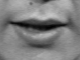
\includegraphics[width=0.15\linewidth]{%
    dataset/avletters/lips_no_data_aug/3}
  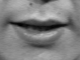
\includegraphics[width=0.15\linewidth]{%
    dataset/avletters/lips_no_data_aug/4}
  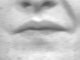
\includegraphics[width=0.15\linewidth]{%
    dataset/avletters/lips_no_data_aug/5}
  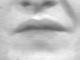
\includegraphics[width=0.15\linewidth]{%
    dataset/avletters/lips_no_data_aug/6}\\[0.15em]
  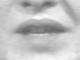
\includegraphics[width=0.15\linewidth]{%
    dataset/avletters/lips_no_data_aug/7}
  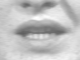
\includegraphics[width=0.15\linewidth]{%
    dataset/avletters/lips_no_data_aug/8}
  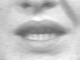
\includegraphics[width=0.15\linewidth]{%
    dataset/avletters/lips_no_data_aug/9}
  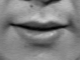
\includegraphics[width=0.15\linewidth]{%
    dataset/avletters/lips_no_data_aug/10}
  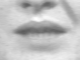
\includegraphics[width=0.15\linewidth]{%
    dataset/avletters/lips_no_data_aug/11}
  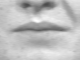
\includegraphics[width=0.15\linewidth]{%
    dataset/avletters/lips_no_data_aug/12}
  \caption{%
    \textbf{Example visual input for the AVletters dataset
      (left to right, top to bottom).}\\[0.1em]
    Pre-extracted lip regions of $60 \times 80$ pixels are provided.
      Each image sequence is resampled to be of length twelve in order to
      give an input of fixed size to the network.}
  \label{fig:avletters_exs}
\end{figure}

\section{Experimental Setup}

To train a classifier I employed the cross entropy cost function and to
train an auto-encoder the L2 distance between the input and output vector
was used as the loss. For the sake of preventing overfitting, L2
regularization \cite{Y. Bengio 2012} was applied to all the weights of
network with a regularization coefficient of $0.0004$.
The Adam algorithm \cite{D. Kingma 2014}
was then introduced for minimizing the loss function.
An exponential decay was further used for the stepsize $\alpha$ of this
algorithm with an initial stepsize $\alpha_0$ varying from 0.01 to 0.0001
depending on experience. The decaying rate $\gamma$
was generally close to 0.8 and
the decay takes place every 100 training steps.

Inputs of the network are normally fed as mini-batches of size 24
(smaller and bigger batch sizes were also experimented).
Batch normalization \cite{S. Ioffe 2015} were introduced after every
convolutional and transposed convoluitonal layer. Therefore, the real
operations used to compute neural activations are more complicated
then what are described above. These settings aren't necessarily optimal
(use a bigger weight regularization coefficient or maybe one had better
use a constant learning rate with Adam optimizer) but I didn't have time
to do more tests on it.

Here are some more details of the network architectures: ReLu
(Rectified Linear Unit) activation were added to all the hidden layers
\cite{A. Krizhevsky 2012} while no activation function was used for
the output layer.
For classification model dropout \cite{N. Srivastava 2014}
was always applied to the second to last layer during training.
The output of the classification layer was mapped to the probabilities
that one data example belongs to each class by the softmax function.

\section{Experiences and Results: Unimodal Cases}

\subsection{Classification}

With every new dataset, I began with training a classifier on it in a
totoally supervised manner.
This gave me an insight into its data quality, the preprocessing
effectiveness and ensured that further experiments could be conducted.
CNN is then one of the most suitable architecture for this purpose.

\subsubsection{Creative Senz3d}

No satisfying results were acquired. It may be due to to a lack of data
quantity, variety, and the fact that the head is also contained in the
image increases significantly the classification difficulty.

\textbf{Subject Dependent.}
In a subject dependant setting, images are separated randomly into
training set (3/4) and test set (1/4). Therefore, during the
testing phase, the classifier doesn't need to deal with data from an
individual that it has never seen before.
In this case, for RGB images, all of the classifiers are able to
have a classification accuracy that is closed to 100\%. This holds true
even for a perceptron.
On the other hand, for depth images, the classification accuracy is
between 60\% and 70\% using a perceptron and near 90\% for other CNN
architectures that were tested.

\textbf{Subject Independant.}
On the contrary, the classifier faces individuals never seen before
during testing in a subject independant setting. 
In my case, the training set consists of images coming from the
first three individuals while the test set contains images of
the final subject.
With the various architectures (including single-layer perceptron
and CNNs varying from three to ten hidden layers)
that I implemented, none of them is able to generalize the learned model
to the new individual.
The pre-trained InceptionV4 architecture achieves a prediction accuracy
of 30\% for color images and 20\% for depth images (better than chance).

\subsubsection{ASL Finger Spelling}

The large number of data contained in this dataset and the relatively
simple image content (single hand instead of the entire upper body)
makes the classification task much easier. By using the CNN architecture
shown in \autoref{fig:CNN10}, we can achieve a classification accuracy
of respectively 80\% and 70\% for intensity and depth images (Table 1)
in an subject-independant setting (four subjects for training and one
subject for testing). We may not need that many layers in the CNN
architecture, but further tests were not carried out since it's not
the essential point of my internship.

\begin{figure}[H]
  \centering
  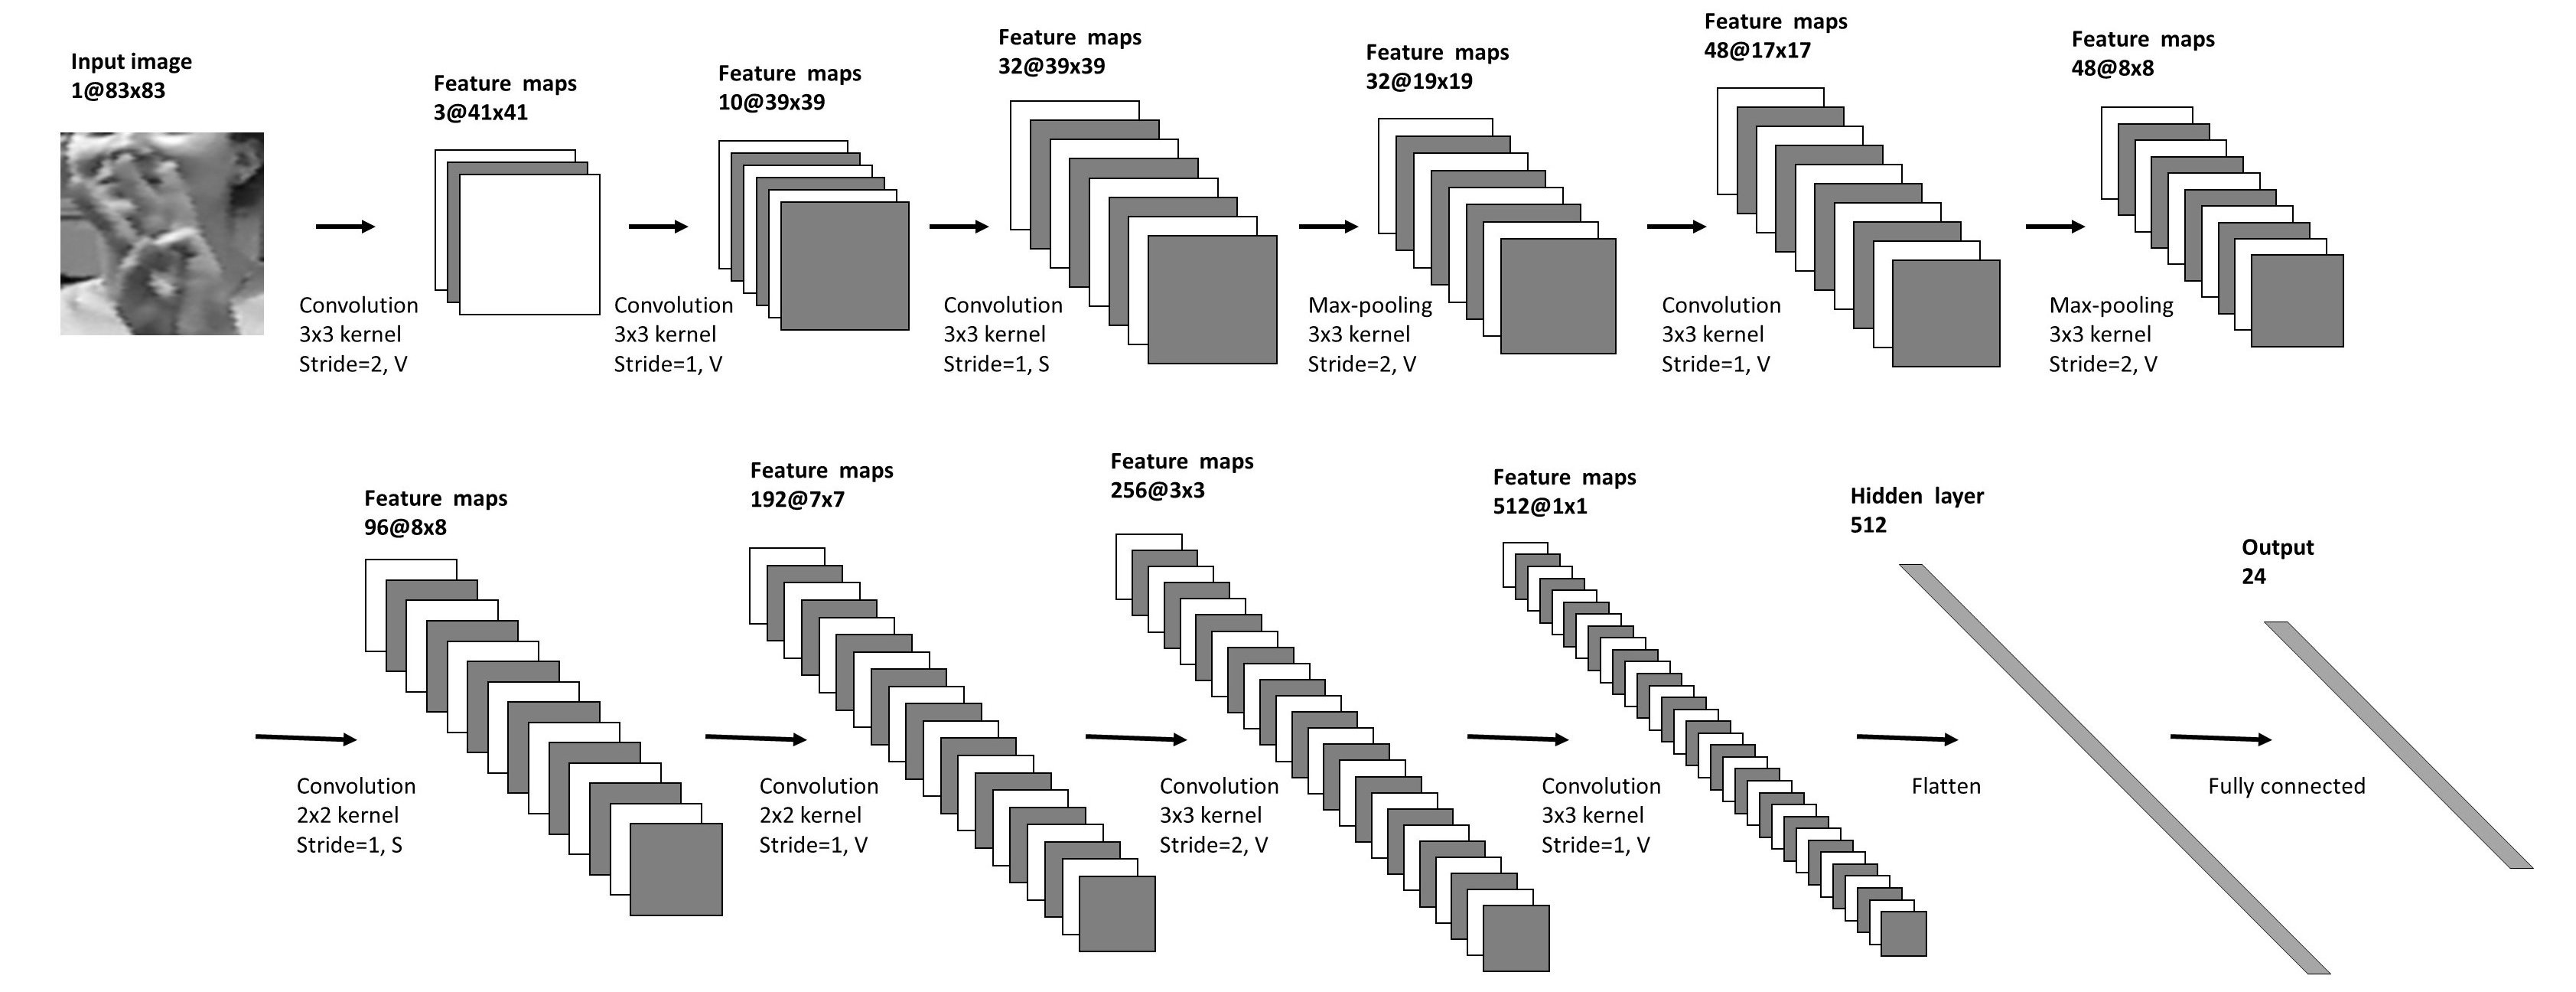
\includegraphics[width=\linewidth]{architectures/CNN10}
  \caption{%
    \textbf{CNN architecture used for the Finger Spelling  dataset.}
      \\[0.1em]
    The input of the nework is a one-channel image of size $83 \times 83$.
      It contains ten hidden layers. S stands for `SAME' padding
      and V stands for `VALID' padding (see text).}
  \label{fig:CNN10}
\end{figure}

\subsubsection{AVletters}

One can refer to \autoref{fig:AVSR_transfer} for the main CNN architectures
that are used in this dataset. 
Notice that 3d CNNs are employed to deal with video inputs.
Considering the small number of available data, a speaker-dependant
setting was used, but it didn't save me from the problem of overfitting.
The classification accuracy is of 100\% for training data but only
of 60\% or 55\% for testing data depending on the input modality
(audio then video).

Curiously, for audio data, I get exactly the same classification
performance regardless of the used architecture (perceptron or CNNs)
or the fact that if deltas and delta-deltas are also given in input.
This is not the case when I test with another audio dataset
(not mentioned in the Datasets and Preprocessing section beacause
it wasn't used for main experiences).
For video input, the use of data augmentation techniques only decrease
the learning speed for the training part but doesn't improve the performace
for testing.

\subsection{Convolutional auto-encoder} \label{subsection:CAE}

Several different CAE architectures were tested in my internship.
Here I present the one with five hidden layers, therefore it contains
three convolutional layers and three transposed convolutional layers
as shown in \autoref{fig:CAE5}. The end-to-end training instead of
a greedy layer-wise approach was used.

The proposed architecture was then trained on the two gesture recognition
datasets. First of all, I'm interested in the denoising capcity of
the auto-encoder. An example is shown in \autoref{fig:image_restoration}.
The auto-encoder is effectively able to reconstruct the clean image in
a way.

\begin{figure}[H]
  \centering
  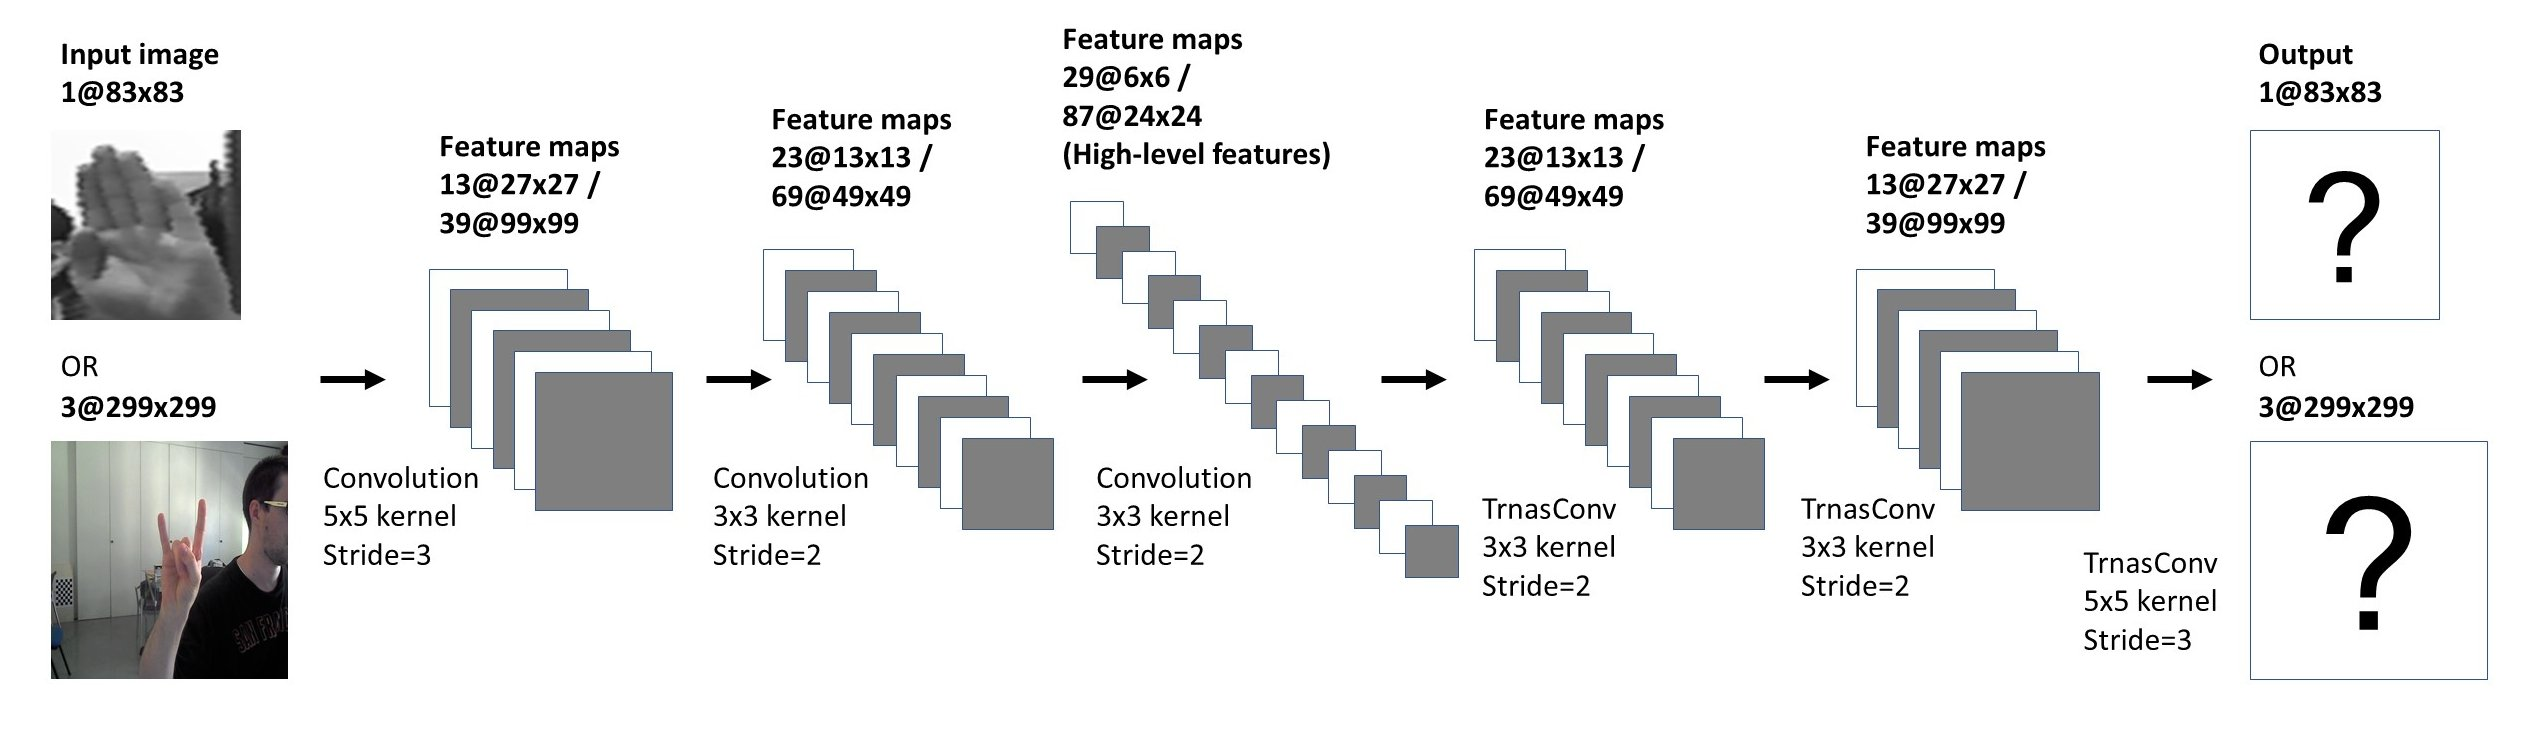
\includegraphics[width=\linewidth]{architectures/CAE5}
  \caption{%
    \textbf{Convolutional auto-encoder architecture with 
      three convolutional layers and three tranposed convolutional
      layer.}\\[0.1em]
    Activation values of the middle layer are taken as 
      high-level features of the input image. Inputs of the network
      can be of different sizes. We only use valid paddings here.}
  \label{fig:CAE5}
\end{figure}

\begin{figure}[H]
  \centering
  \hfill
  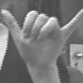
\includegraphics[width=0.28\linewidth]{%
    dataset/fingerspelling5/gray/gray4}
  \hfill
  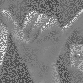
\includegraphics[width=0.28\linewidth]{%
    dataset/fingerspelling5/gray/gray_dropout4}
  \hfill
  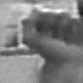
\includegraphics[width=0.28\linewidth]{%
    dataset/fingerspelling5/gray/gray_reconstruction4}
  \caption{%
    \textbf{Image restoration using convolutional auto-encoder.}\\[0.1em]
      Left) Clean Image.\\[0.1em]
      Middle) Noisy image [input].\\[0.1em]
      Right) Restored image [output].}
  \label{fig:image_restoration}
\end{figure}

\section{Experiences and Results: Multimodal Cases}

\subsection{Learning shared representation}

\begin{figure}[H]
  \centering
  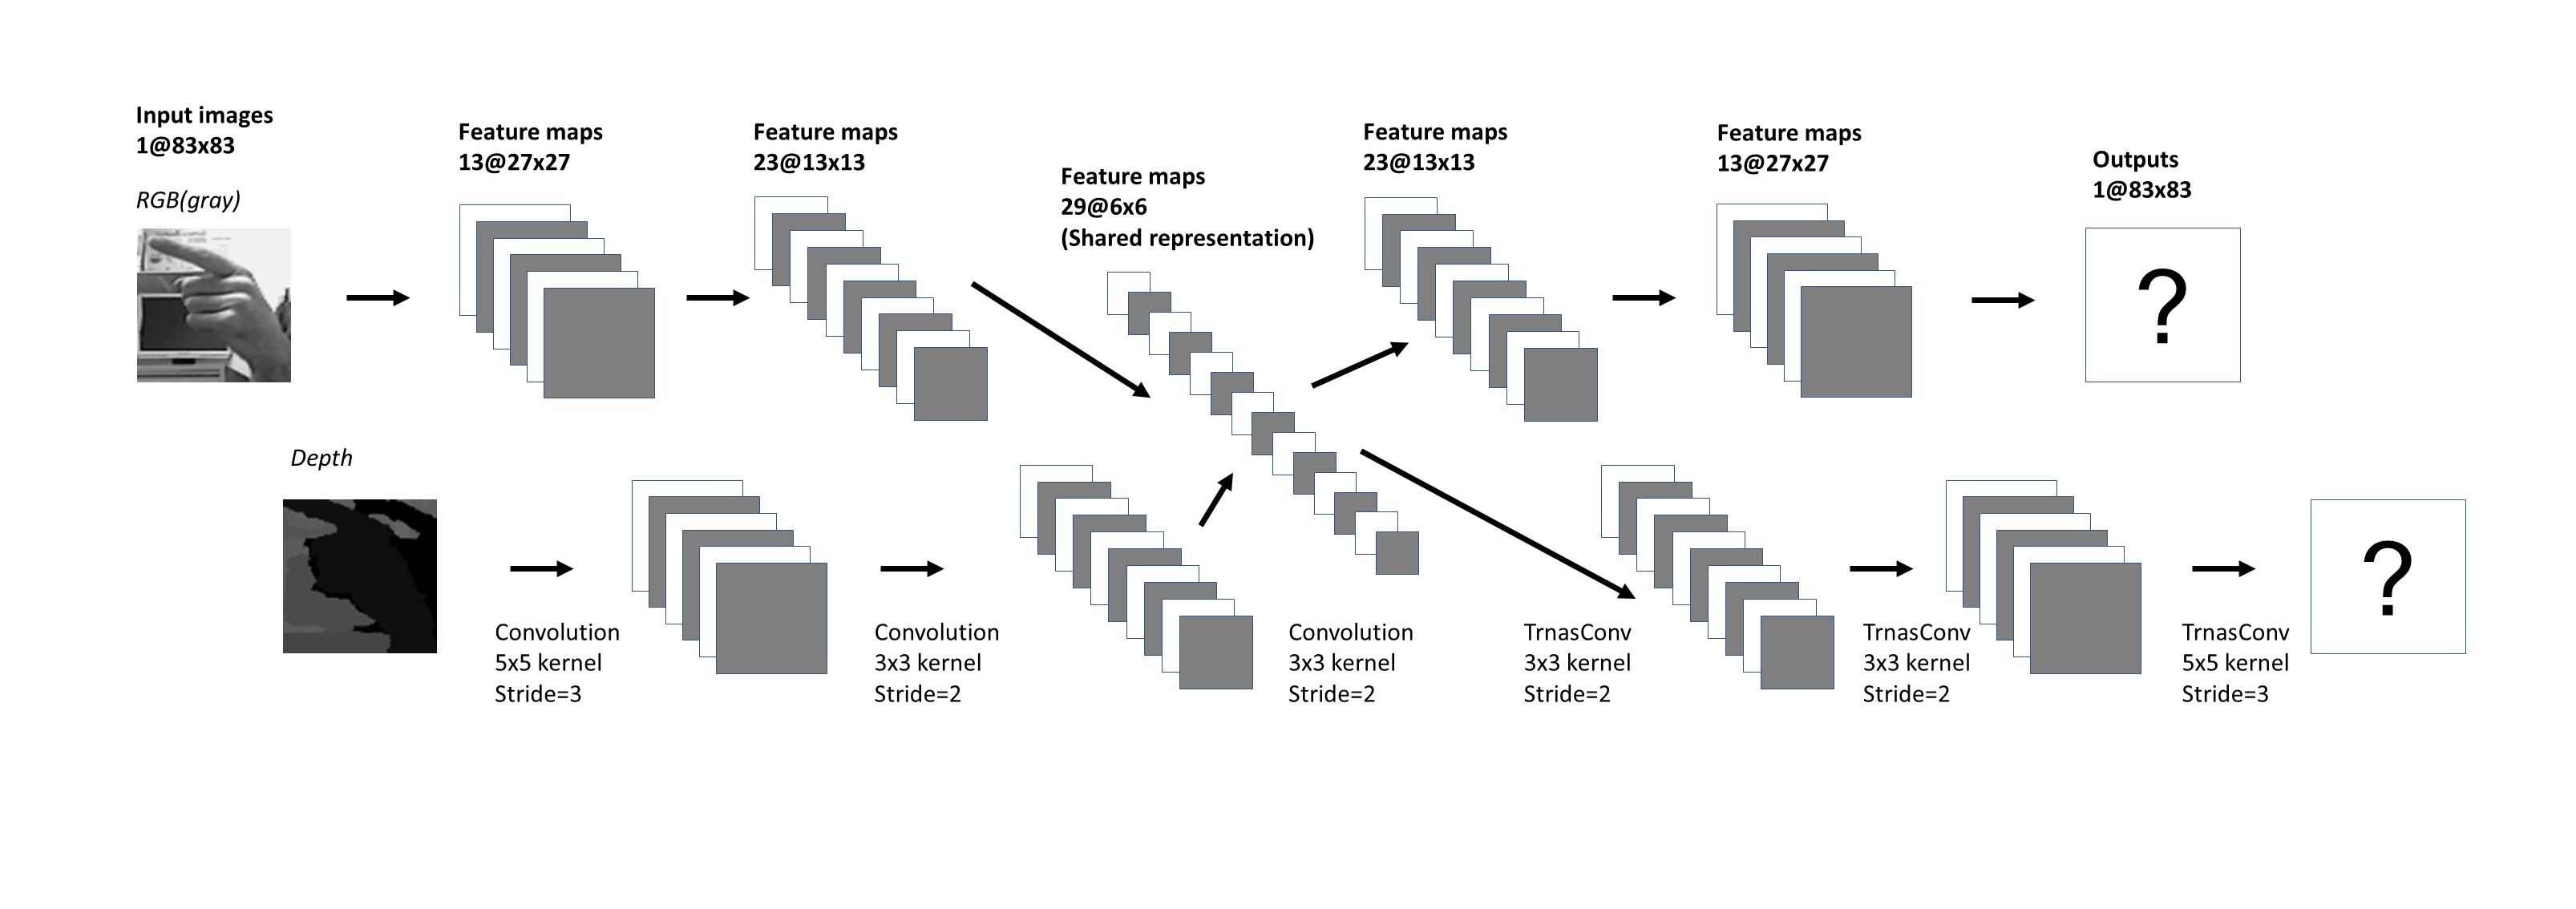
\includegraphics[width=\linewidth]{architectures/FAE5}
  \caption{%
    \textbf{The bimodal convolutional auto-encoder model that is
      used to learn shared multimodal representation.}\\[0.1em]
    We simply take the CAE architecture that is introduced earlier
      (\autoref{fig:CAE5}) for each modaliy but force them to have a
      shared middle layer by adding the corresponding activation values.
      We then try to reconstruct the two images separately through
      two disjoint paths.}
  \label{fig:FAE5}
\end{figure}

\begin{figure}[H]
  \centering
  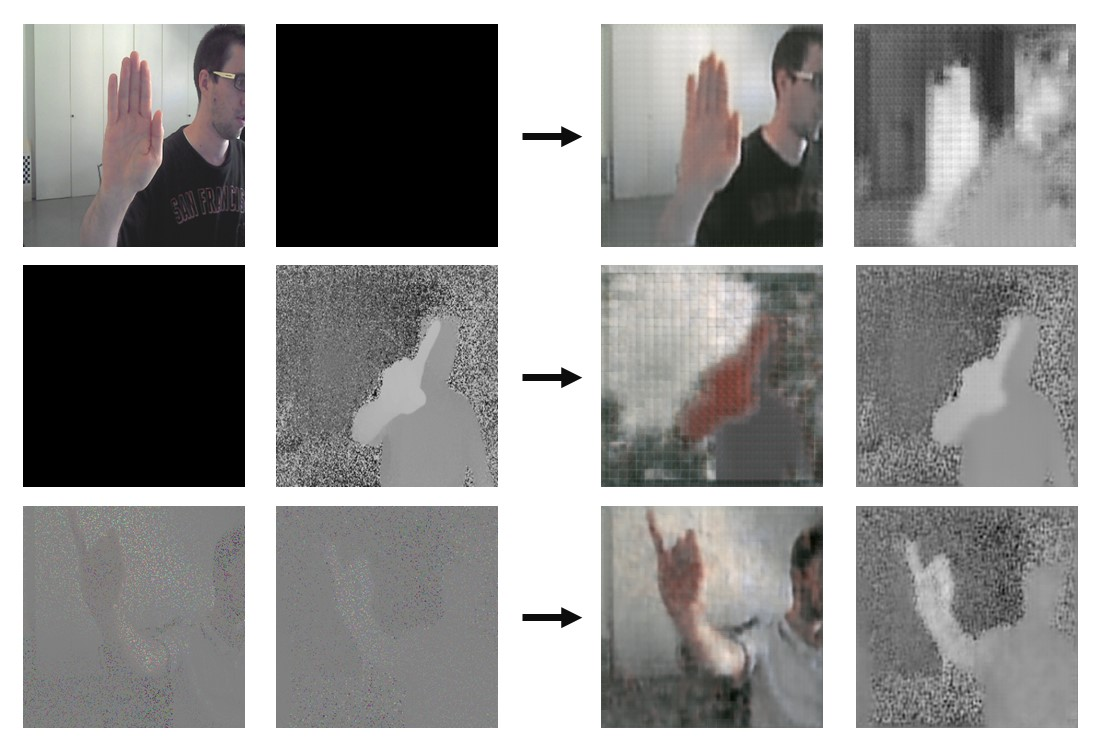
\includegraphics[width=\linewidth]{dataset/senz3d/reconstructions}\\[-1em]
  \caption{%
    \textbf{Restore color and depth images from incomplete input
      information.}\\[0.1em]
    Top) Only the color image is given.\\[0.1em]
    Middle) Only the depth image is given.\\[0.1em]
    Botttom) Both modalities are given but with little information
      (10\% of pixels).}
  \label{fig:color_depth_restoration}
\end{figure}

\begin{table}
  \tabcolsep = 9pt
  \begin{tabular*}{\linewidth}{>{\bf}llccccc}
    \toprule
    && Raw & CAE features & Shared & CAE architecture & CNN\\
    \midrule
    \multirow{2}{*}{Intensity} &
    train & 69.47 \% & 78.39 \% & 81.07 \% & 92.34 \% & 99.69 \% \\
    & test & 32.64 \% & 50.72 \% & 50.92 \% & 67.23 \% & 79.73 \% \\
    \midrule
    \multirow{2}{*}{Depth} &
    train & 48.17 \% & 38.65 \% & 73.07 \% & 90.4 \% & 97.24 \% \\
    & test & 30.95 \% & 26.39 \% & 43.50 \% & 58.69 \% & 66.84 \% \\
    \midrule
    \multirow{2}{*}{Depth (Z-n)} &
    train & 63.64 \% & 72.37 \% & 72.01 \% &  \% & 97.24 \% \\
    & test & 29.93 \% & 40.03 \% & 40.27 \% &  \% & 64.46 \% \\
    \bottomrule
  \end{tabular*}
\end{table}

\subsection{Transfer learning}

\begin{figure}[H]
  \centering
  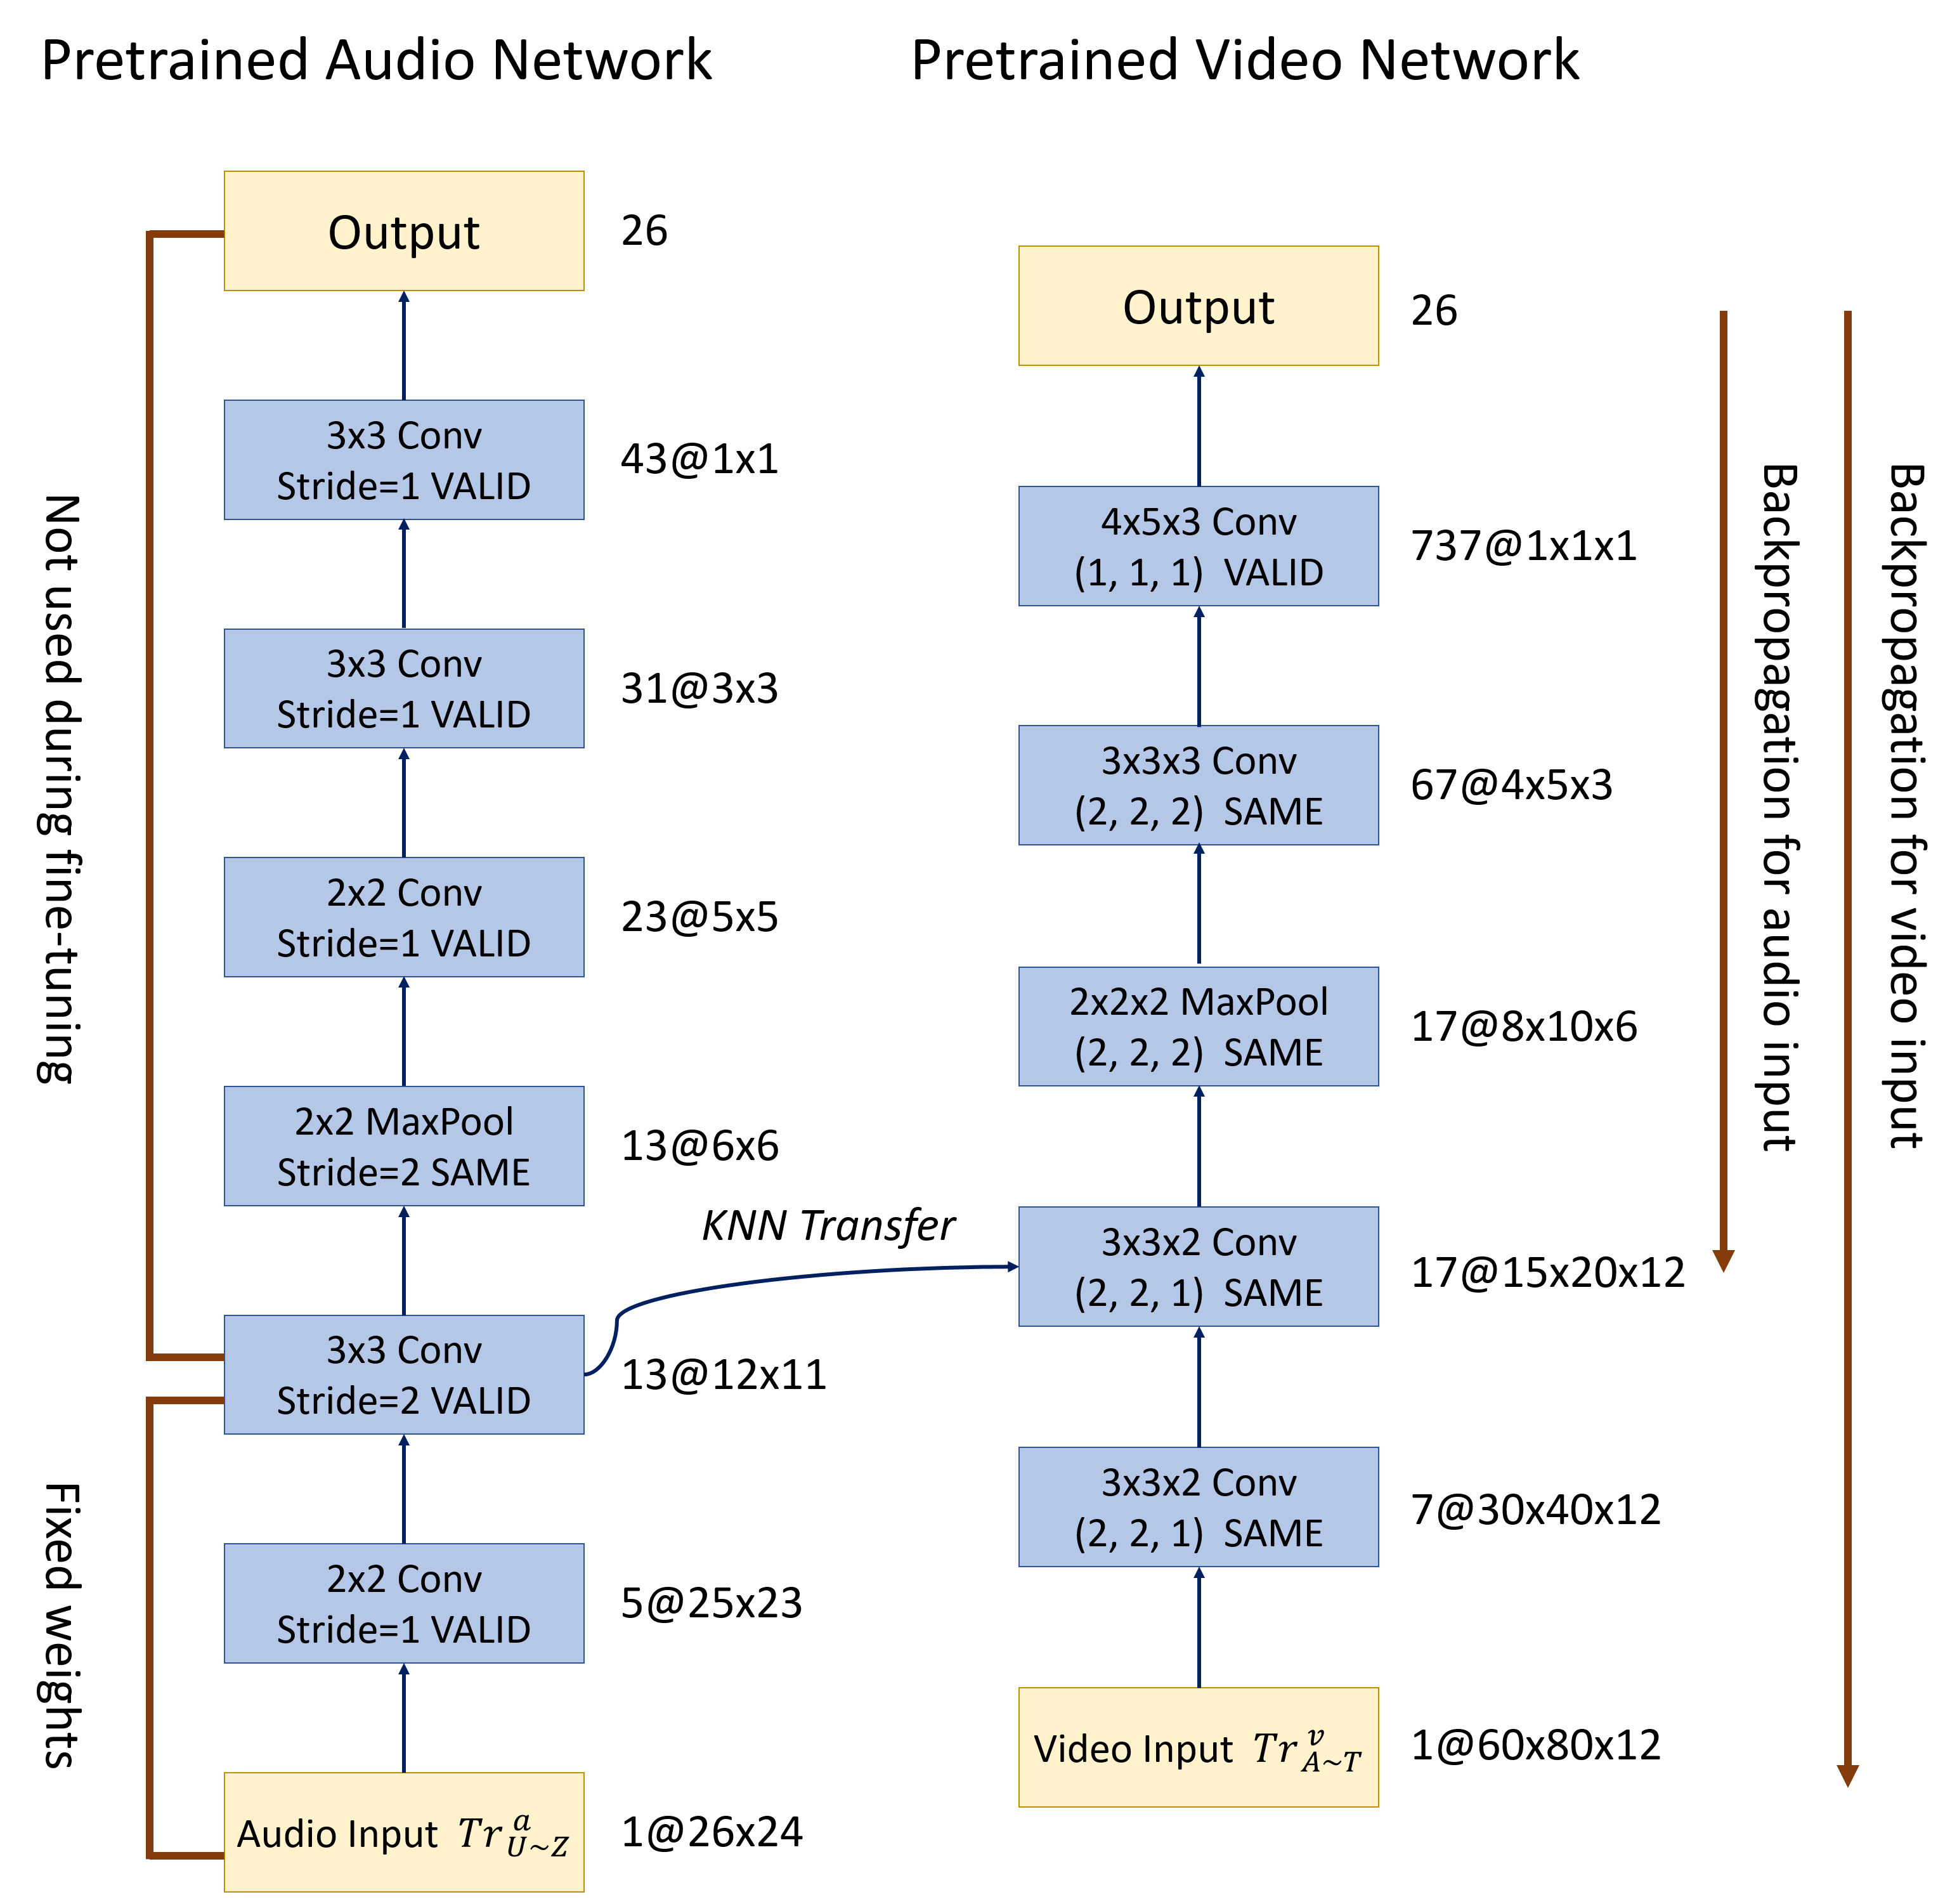
\includegraphics[width=0.9\linewidth]{architectures/AVSR_transfer}\\[-1em]
  \caption{%
    \textbf{Illustration of the transfer learning approach applied in
      audio and lip-reading speech recognition tasks.}\\[0.1em]
    We first learn two separated model for audio and visual inputs
      (in my cases two CNNs) and try to fine-tune the video network
      with transferred audio data.
    }
  \label{fig:AVSR_transfer}
\end{figure}
